\documentclass[11pt]{article}
\usepackage{theme}
\usepackage{shortcuts}
\usepackage{listings}
\usepackage{hyperref}
\usepackage{minted}
\usepackage{subcaption}
% \usepackage[backend=biber]{biblatex}
% \addbibresource{references.bib}
% Document parameters
% Document title
\title{Mini-Project (ML for Time Series) - MVA 2024/2025}
\author{
Alexis Marouani \email{alexis.marouani@polytechnique.edu} \\ % student 1
Grégoire Béchade \email{gregoire.bechade@polytechnique.edu} % student 2
}

\begin{document}
\maketitle

% \paragraph{What is expected for these mini-projects?}
% The goal of the exercise is to read (and understand) a research article, implement it (or find an implementation), test it on real data and comment on the results obtained.
% Depending on the articles, the task will not always be the same: some articles are more theoretical or complex, others are in the direct line of the course, etc... It is therefore important to balance the exercise according to the article. For example, if you have reused an existing implementation, it is obvious that you will have to develop in a more detailed way the analysis of the results, the influence of the parameters etc... Do not hesitate to contact us by email if you wish to be guided.

% \paragraph{The report}
%  The report must be at most FIVE pages and use this template (excluding references). If needed, additional images and tables can be put in Appendix, but must be discussed in the main document. The report must contain a precise description of the work done, a description of the method, and the results of your tests. Please do not include source code! The report must clearly show the elements that you have done yourself and those that you have reused only, as well as the distribution of tasks within the team (see detailed plan below.)
 
%  \paragraph{The source code}
% In addition to this report, you will have to send us a Python notebook allowing to launch the code and to test it on data. For the data, you can find it on standard sites like Kaggle, or the site https://timeseriesclassification.com/ which contains a lot of signals!


% \paragraph{The oral presentations}
% They will last 10 minutes followed by 5 minutes of questions. The plan of the defense is the same as the one of the report: presentation of the work done, description of the method and analysis of the results.


% \paragraph{Deadlines}
% Two sessions will be available :
% \begin{itemize}
%  \item \textbf{Session 1}
%  \begin{itemize}
%   \item Deadline for report: December 18th (23:59)
%   \item Oral presentations: December 19th and 20th (precise times TBA)
%  \end{itemize}
% \item \textbf{Session 2}
%  \begin{itemize}
%   \item Deadline for report: January 8th (23:59)
%   \item Oral presentations: January, 9th and 10th (precise times TBA)
%  \end{itemize}
% \end{itemize}

\section{Introduction and contributions}
The paper we studied aims to introduce a novel method to perform anomaly detection in large time series, based on the introduction of a "normal behaviour" of the time series.
Anomaly detection can be defined in several manners. 
It can be interpreted as "outlier detection", where the objective is to detect single anormal points (which can for instance correspond to sensor failures). 
The paper focuses on the second type of task, which aims to detect anormal subsequences of the time series. 
In this case, several consecutive points behave anormaly (for instance, an anormal heartbeat or an anormal day of electricity consumption).
The authors decided to consider that an anomaly sequence is a sequence that can be observed several times in the time-series, in opposition to another definition that would consider an anomaly as a unique sequence.
The method aims to define the expected behaviour of the time series, and defines anomalies as subsequences that are too far from this expected behaviour.
The real contribution of this new method is not an improvment in terms of accuracy, but in computational time. 
Indeed, the approximation of the expected behaviour prevents to compute the distances between all pairs of subsequences. \\[0.5cm]
We decided to reproduce the algorithm described in the paper, to implement some variations, and test it on new data. \\[0.5cm]
We decided to split the work as follows : Grégoire made the data extraction and vizualization and Norma1. Alexis did Norma2 and our personal variation. \\[0.5cm]
As the source code was not available, we reimplemented everything ourselves. \\[0.5cm]
Experiments: Several algorithms from the original papers were run, and our own variation using k-means instead of hierarchical clustering was implemented. 
A new method to sample the subsequence was also tested and significantly improves the results. \\[0.5cm]




% The Introduction section (indicative length : less than 1 page) should detail the scientific context of the article you chose, as well as the task that you want to solve (especially if you apply it on novel data). \textbf{The last paragraph of the introduction must contain the following information}:
% \begin{itemize}
%     \item Repartition of work between the two students
%     \item Use of available source code or not, percentage of the source code that has been reused, etc.
%     \item Use of existing experiments or new experiments (e.g. test of the influence of parameter that was not conducted in the original article, application of the method on a novel task/data set etc.)
%     \item Improvement on the original method (e.g. new pre/post processing steps, grid search for optimal parameters etc.)
% \end{itemize}

\section{Method}

Classical methods for anormal sequences detection rely on the fact that anormal sequences are considered as unique sequences in the time-series. 
These methods label as anomalies the sequences that are far away from every other subsequence of the time series, for a given metric (euclidian, DTW for instance). 
However, as explained in the article, one can be looking for anomalies that are not unique, like anormal heartbeats in a ECG.
The method proposed introduces the \textbf{normal model} ($N_M$), which is a sequence of fixed length (here $3 \times l $, with $l$ the length of the anomalies we are looking for), that represents the "normal behaviour" of the model. 
The proposed method to determine the $N_M$ is : 
\begin{enumerate}
    \item Extract the subsequences of length $3 \times l$  (randomly or with motif selection). 
    \item Perform a hierarchical clustering of the subsequences.
    \item Select the cluster $c$ in $\mathbb{C}$ (the set of clusters) that maximises the following quantity : $N(c) = \frac{frequency (c)^2 \times coverage (c) }{ \Sigma_{x \in \mathbb{C} } dist(center(c), center(x))}$\\
    With $frequency(c)$ the number of sequences in the cluster, $coverage(c)$ the time lag between the first and the last sequences in the cluster, and $center(c)$ the barycenter of the cluster.
    This quantity aims to select the cluster with the most sequences, and that is close to all the other clusters. 
    \item Finally, $N_M$ is defined as the barycenter of the cluster $c$.
\end{enumerate}

The distance of a subsequence to the normal model is then defined as the minimal (euclidian) distance between a subsequence os size $l$ and all the subsequences in the normal model of size $l$ (as a recall, the normal model is of size $3 \times l$).
The authors describe several metric to label a subsequence as \textit{anormal}. 
Selecting the $k$ subsequences with the biggest minimal distance to the normal model, or selecting the ones that are above a certain threshold can be methods to determine the anomalies.

The key point of the method is that instead of comparing an anomaly to all the subsequences of the time-series and then comparing it to a very large number of identical pattern, the clustring step enables to drastically reduce the number of comparisons. 
Indeed, each sequence of size $l$ is compared to $2 \times l $ sequences in the normal model, instead of $T - 2 \times l$ in the whole time series (with the condition of non overlap). 


We decided to implement the algorithm from scratch to try to reproduce the results from the paper. 

A first implementation was tested, trying to reproduce exactly the algorithm from the paper (\textbf{Norma1 without seasonal sampling}). \\[0.5cm]

\textbf{Seasonal sampling : }\\
We noticed that the sampling was not optimal, as sequences beginning at different hours were compared with an euclidian distance, which did not seem relevant.
For the other algorithms described above, we decided to perform a samplig which took into account the seasonality of the time series as follows : 
We randomly selected approximately 50 subsequences of size $ 7 \times 48 = 336$ from the original time-series. 
Indeed, as the final step of the clustering consists in determining a barycenter, and as there is a strong seasonality in the time series, we don't want to sum a subsequence beginning at 7:00 and a subsequence beginning at 23:00, as it would probably converge toward a flat distribution. 
The sampling was then performed on days, in order to have subsequences beginning at the same time. 

We decided to fix a size of 7 days for the normal model to catch a "normal week". 

Three algorithms were tested with this seasonal sampling :

\begin{enumerate}
    \item First, we tried to reproduce the algorithm from the paper, with hierarchical clustering and selecting the centroïd of the most representative cluster as the normal model, as explained above (\textbf{Norma1 with seasonal sampling}).\\
    \item Then, we tried another algorith from \ref{ref1}, which follows the same method but decides to define as the normal model the average mean of the centroids of each cluster, with the score of each cluster as weights (\textbf{Norma2 with seasonal sampling}). 
        This approach aims at better catching the normal behaviour of the time series. 
        Indeed, if there is two normal patterns with a very different shape in the time series, the first approach would label as anomaly every pattern of the second size, while the second approach integrates this information. \\
    \item   Finally, we implemented our own variations, with the use of k-means instead of hierarchical clustering. 
            The first variation gets the centroid of the most representative cluster as the normal model (\textbf{K-means variation 1 with seasonal sampling}), as it is done in Norma1. 
            The second variation defines the normal model as the averaged sum of the centroids of each cluster with respect to the criterion defined above (\textbf{K-means variation 2 with seasonal sampling}), as it is done in Norma2. 

\end{enumerate}




To evaluate our model, we computed the score of each subsequence of the origin time-series, defined as the minimal distance between this subsequence and each subsequence in the normal model, and selected the 10 most anormal subsequences.

% The Method section (indicative length : 1 to 2 pages) should describe the mathematical aspects of the method in a summarized manner. Only the main steps that are useful for understanding should be highlighted. If relevant, some details on implementation can be provided (but only marginally).

\section{Data}

We decided to run the algorithm on the NYC taxis dataset, which represents the number of calls to taxis in New York City every 30 minutes between 01/07/2014 and 30/01/2015, available \href{https://github.com/numenta/NAB/blob/master/data/realKnownCause/nyc_taxi.csv}{here}. 
The dataset has 5 anomalies highlighted, that we aim to detect. 
This dataset seemed performant because of its big size : 10320 points. 
Its mean is 15137.57, with a standard deviation of 6931.92. \\
The figure \ref{fig:taxis} shows a day of the time-series.
\begin{figure}[h]
    \centering
    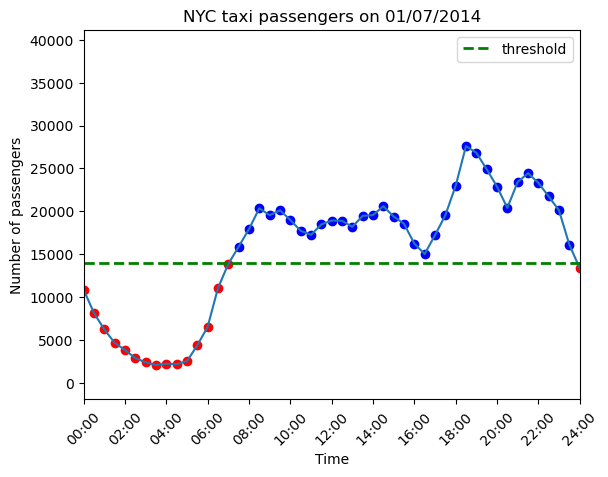
\includegraphics[width=0.5\textwidth]{example_day.png}
    \caption{A day of the NYC taxis dataset}
    \label{fig:taxis}
\end{figure}

\begin{figure}[h]
    \centering
    \begin{subfigure}[b]{0.45\textwidth}
        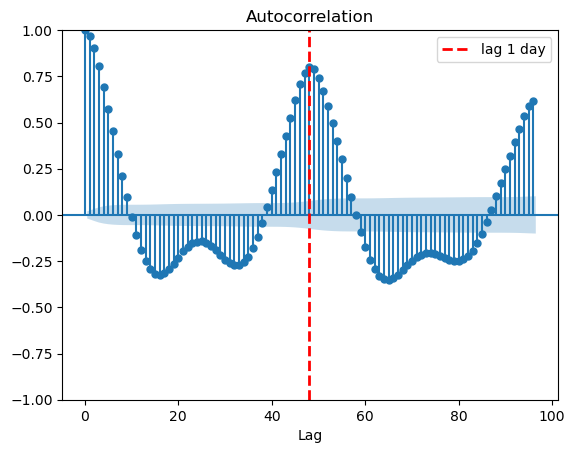
\includegraphics[width=\textwidth]{autocorrelation.png}
        \caption{Autocorrelation plot}
        \label{fig:autocorrelation}
    \end{subfigure}
    \hfill
    \begin{subfigure}[b]{0.45\textwidth}
        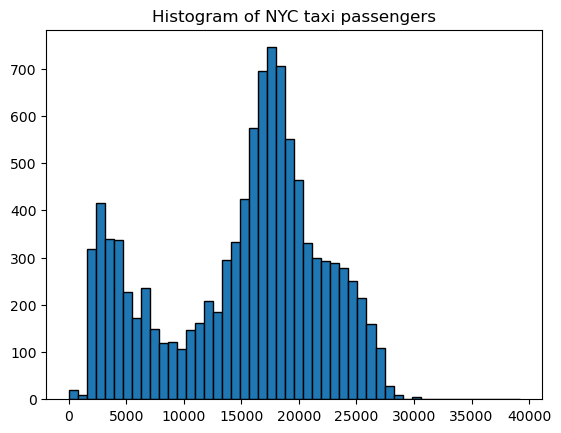
\includegraphics[width=\textwidth]{histograms.png}
        \caption{Histogram of values}
        \label{fig:histograms}
    \end{subfigure}
    \caption{Data analysis}
    \label{fig:data_analysis}
\end{figure}
Augmented Dicky-Fuller and KSS tests showed p-values of respectively 2.5e-19 and 0.06, which confirms the stationarity of the time-series. 
The periodicity of the time-series was confirmed by an autocorrelation plot  (see Fig.\ref{fig:autocorrelation}), with a peak every 48 points, corresponding to 24 hours time-lag. 
An histogram of the values taken by the time-series shows a bimodal distribution with few outliers, separated by the 14000 value (see Fig.\ref{fig:histograms}). 
Values below 14000 correspond almost exactly to hours between 00:00 and 07:00, which is coherent with the physical meaning of the time-series (see figure \ref{fig:taxis}).


% The Data section (indicative length : 1 page) should provide a deep analysis of the data used for experiment. In particular, we are interested here in your capacity to provide relevant and thoughtful feedbacks on the data and to demonstrate that you master some "data diagnosis" tools that have been dealt with in the lectures/tutorials.

\section{Results}
The three algorithms described in the methods were run on the taxi dataset. 
10 anomalies were extracted, and the goal was to detect the 5 known anomalies in the dataset. 
First, one can notice that Norma1 has better results with seasonal sampling rather than random sampling, as can be noticed on the score curve, whose variance diminishes with seasonal sampling. 
Norma 1 and Norma 2 with seasonal sampling returns roughly the same results, and identify correctly the 5 anomalies which correspond to aldready detected anomalies in the time-series (Thanksgiving and Christmas leading to a huge increase in the number of calls to join the family at unexpected hours and New-York marathon or a snow storm leading to a decrease in the number of calls). 
New anomalies were also detected by those two algorithms.
\ref{ref1} also pointed out these new anomalies, and observed that they corresponded to very rainy days. 
The method seems relevant, as it enabled to detect new anomalies. 
One can also notice that the anomaly score is less regular in the Norma1, which is a good thing, as sundays should not be more anormal than mondays. 
The k-means variations algorithms do not manage to catch the expected anomalies. 
To conclude, Norma1 with seasonal variations algorithm outperforms the other algorithms tested. 
% The Result section (indicative length : 1 to 2 pages) should display numerical simulations on real data. If you re-used some existing implementations, it is expected that this section develops new experiments that were not present in the original article. Results should be discussed not only based on quantative scores but also on qualitative aspects. In particular (especially if your article focuses on black box methods), please provide some feedbacks whether the method was adapted to the data or not and whether the hypothesis behind the approach you used were validated or not.

\begin{figure}[h]
    \centering
    \begin{subfigure}[b]{0.35\textwidth}
        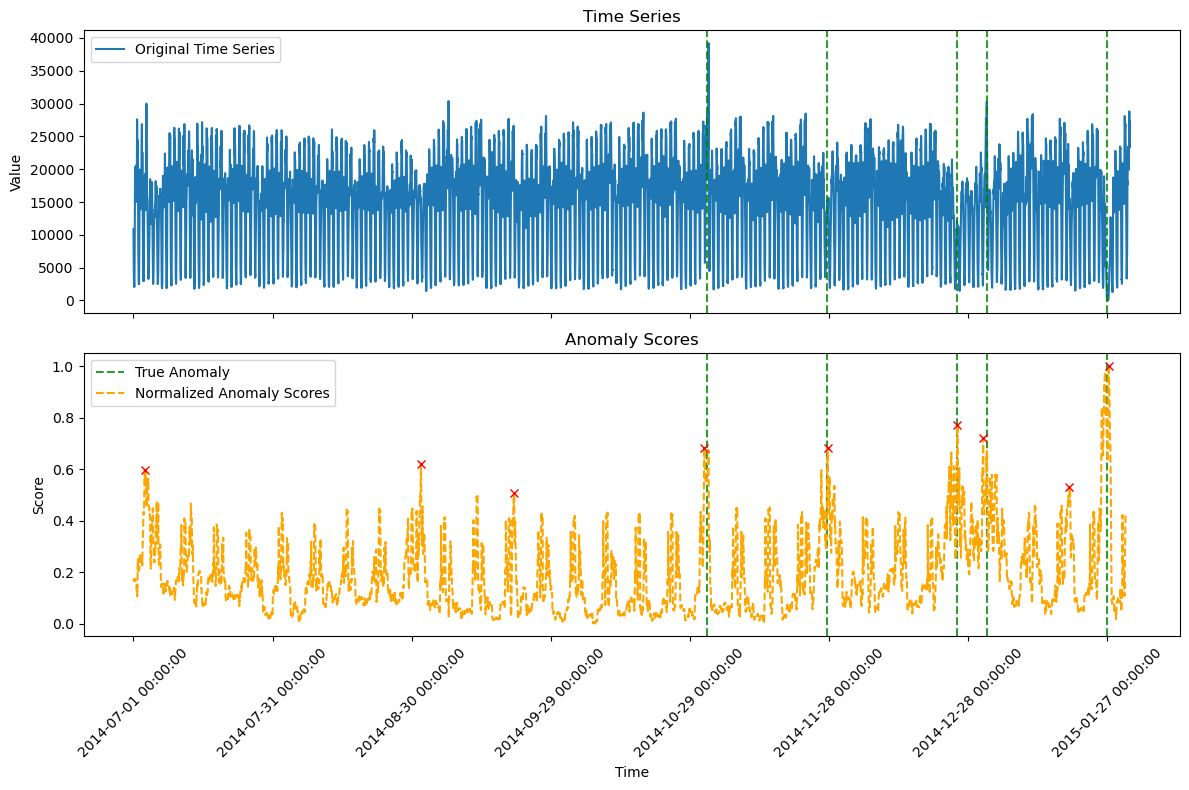
\includegraphics[width=\textwidth]{algo0.jpg}
        \caption{Results from Norma1 with random sampling}
        \label{fig:algo0}
    \end{subfigure}

    \begin{subfigure}[b]{0.35\textwidth}
        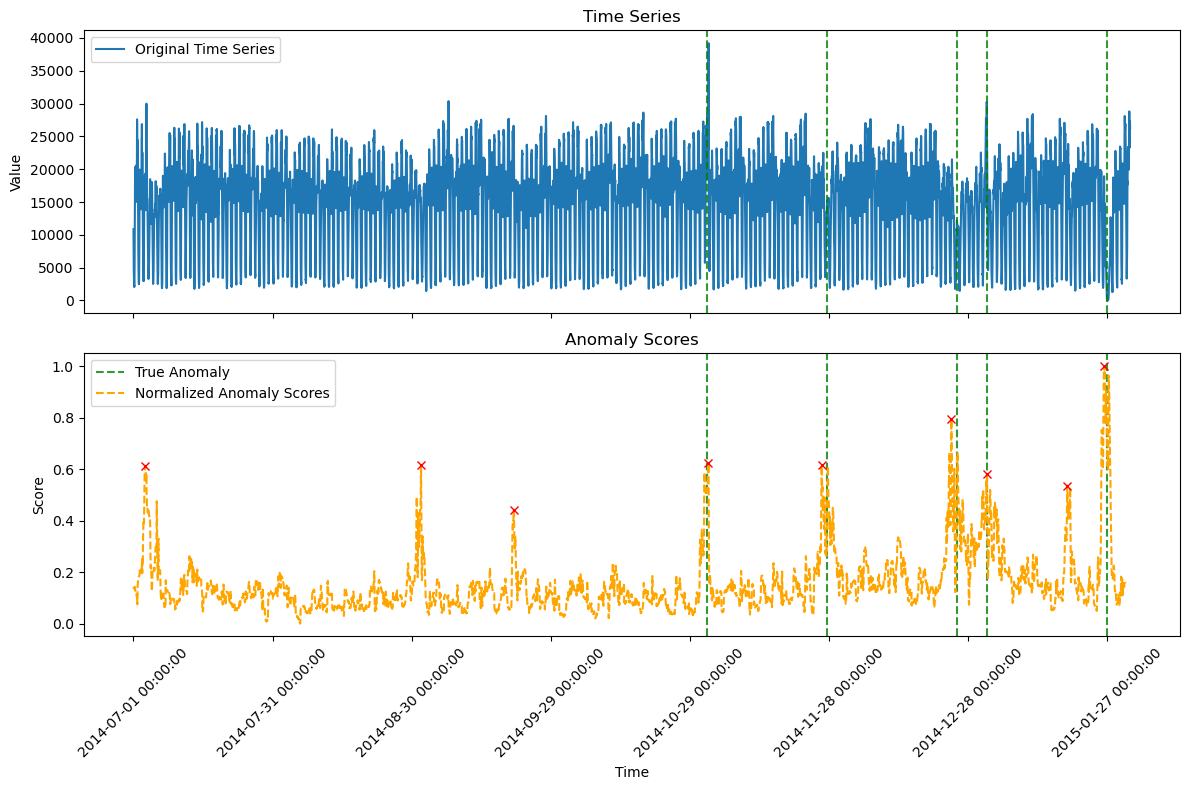
\includegraphics[width=\textwidth]{algo1.png}
        \caption{Results from Norma1 with seasonal sampling}
        \label{fig:algo1}
    \end{subfigure}

    \begin{subfigure}[b]{0.35\textwidth}
        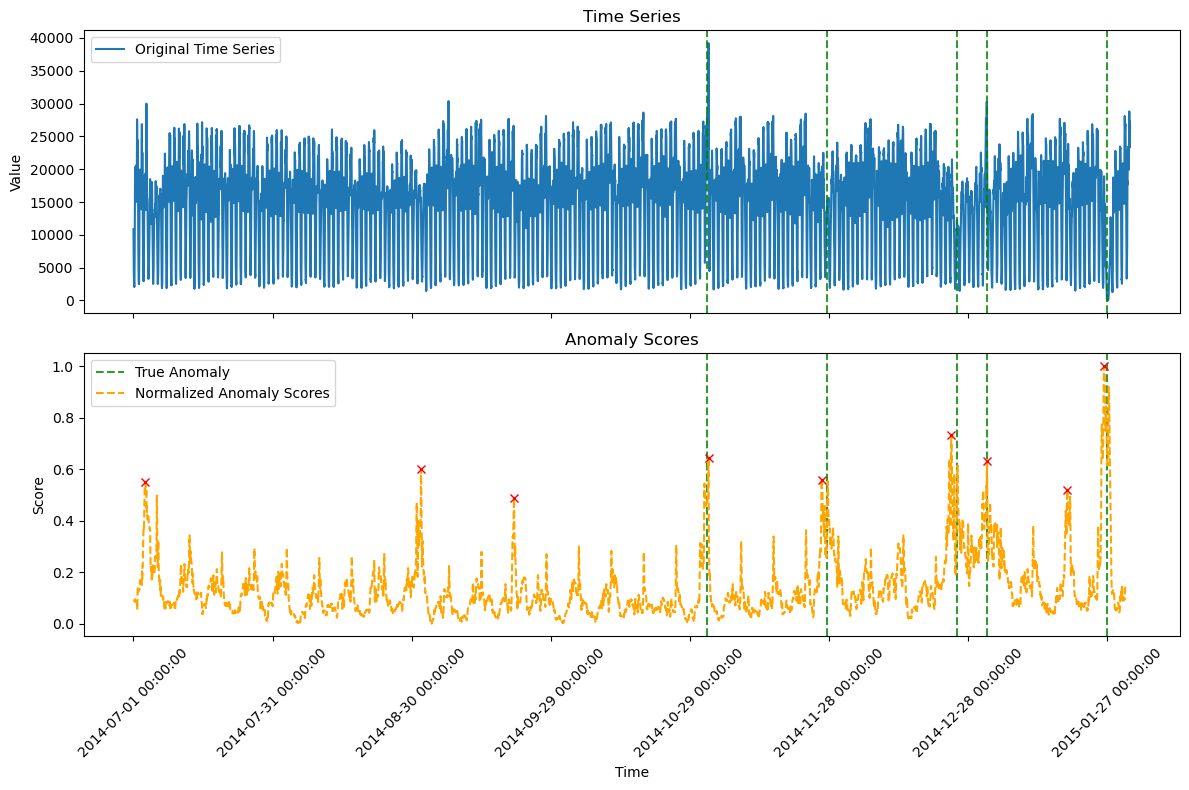
\includegraphics[width=\textwidth]{algo2.png}
        \caption{Results from Norma2 with seasonal sampling}
        \label{fig:algo2}
    \end{subfigure}

    \begin{subfigure}[b]{0.35\textwidth}
        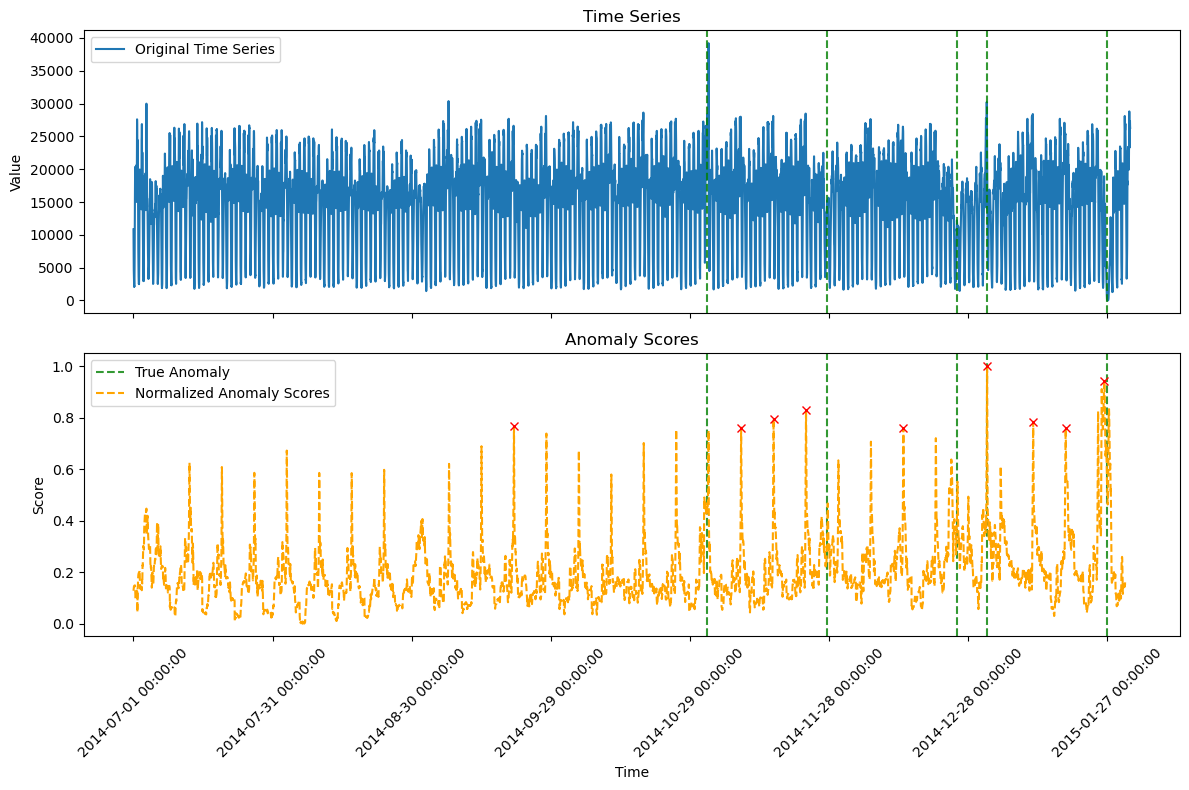
\includegraphics[width=\textwidth]{algo3.png}
        \caption{Results from k-means variation 1 with seasonal sampling}
        \label{fig:algo3}
    \end{subfigure}

    \begin{subfigure}[b]{0.35\textwidth}
        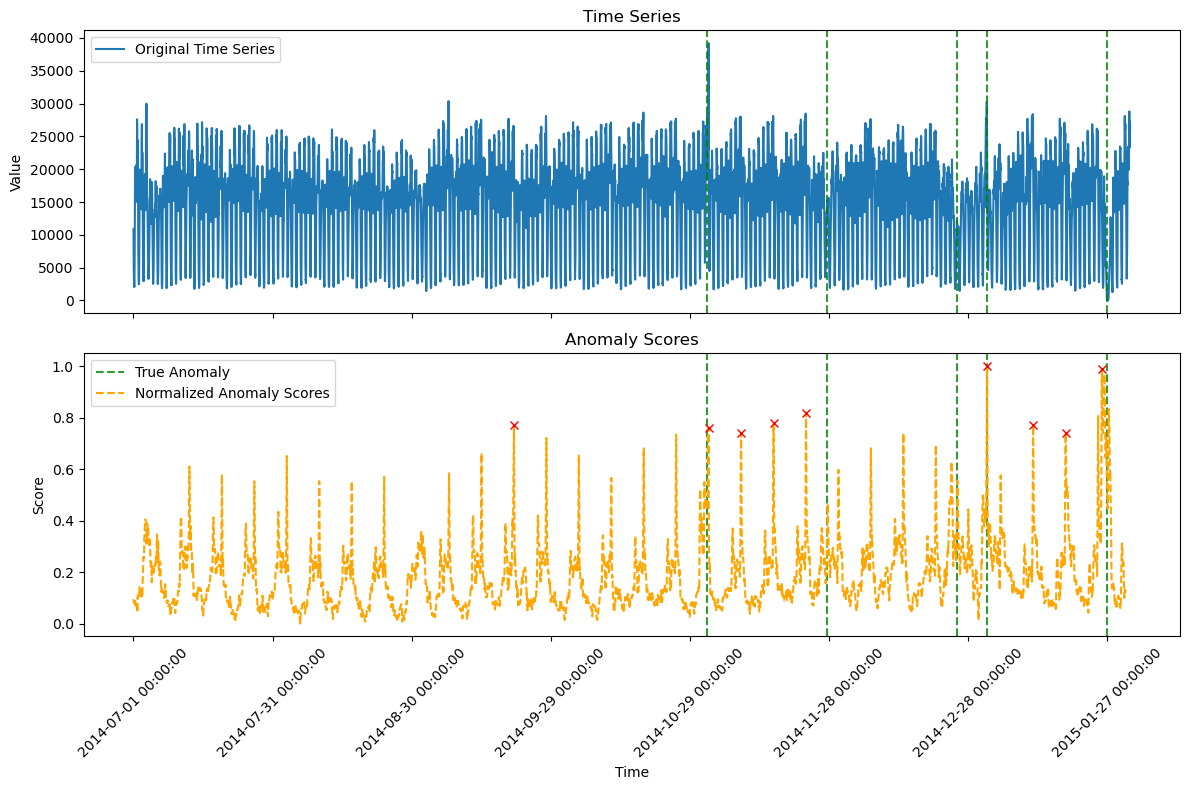
\includegraphics[width=\textwidth]{algo4.png}
        \caption{Results from k-means variation 2 with seasonal sampling}
        \label{fig:algo3}
    \end{subfigure}
    \caption{Results of the different algorithms}
    \label{fig:results}
\end{figure}



% references
\section{References}
\label{ref1} Boniol, P., Linardi, M., Roncallo, F., Palpanas, T., Meftah, M., \& Remy, E. (2021). Unsupervised and scalable subsequence anomaly detection in large data series. The VLDB Journal, 30(6), 909-931.

\end{document}
